\section{Simulation study}
\label{sec:simulation}

\subsection{Design}

We assessed the finite-sample performance of the SAFH estimator in a
model-based simulation designed to mimic the application. In each scenario we
generated $m$ districts with remoteness values $r_i$ drawn from a gamma
distribution with shape 2 and scale 0.9, truncated at 8 hours, which reproduces
the right-skewed distribution of travel times observed in the NPHNS districts.
Two additional covariates were generated as $x_{i1} \sim N(0, 1)$ and
$x_{i2} \sim \mathrm{Bernoulli}(0.4)$, and the district prevalences were
generated as
\begin{equation}
  \theta_i = 0.18 + 0.03\, x_{i1} - 0.02\, x_{i2} + f_s(r_i) + u_i,
  \qquad u_i \sim N(0, \sigma_u^2),
  \label{eq:sim}
\end{equation}
for three mean functions: a linear function $f_1(r) = 0.03\, r$, a concave
function $f_2(r) = 0.12\{1 - \exp(-0.9 r)\}$ and a step function
$f_3(r) = 0.08\, \mathbb{1}\{r > 2.5\}$. The area-level variance took the values
$\sigma_u^2 = 0.0004$ (low) and $\sigma_u^2 = 0.0016$ (high), and the number of
districts was $m = 50$ or $m = 100$, giving twelve scenarios in total. The
sampling variances were set to $\psi_i = \theta_i(1 - \theta_i)\, d / n_i$ with
a design effect $d = 1.8$ and district sample sizes $n_i$ drawn from the
empirical distribution of the NPHNS district sample sizes. The values of
$\psi_i$ were held fixed across the $R = 1000$ Monte Carlo replicates of each
scenario.

We compared three estimators: the standard Fay--Herriot EBLUP with $r_i$
entering linearly (FH), the Fay--Herriot EBLUP with $\log(1 + r_i)$ in place of
$r_i$ (FH-log), and the proposed SAFH estimator with $K = \min\{\lfloor m/4 \rfloor, 35\}$ knots.
All variance components were estimated by REML. For each estimator we recorded
the root mean squared error (RMSE) and the absolute relative bias, averaged over
districts, and for SAFH the coverage and average width of nominal 95\% bootstrap
intervals.

\subsection{Results}

Table~\ref{tab:sim} summarizes the RMSE of the three estimators and the coverage
of the SAFH intervals. When the true mean function is linear, the three
estimators perform almost identically; the SAFH estimator pays a small price for
estimating the additional variance component, and its RMSE is slightly larger
than that of the FH estimator in the two scenarios with $m = 50$. In all other
scenarios SAFH has the smallest RMSE, so that it improves on the standard
estimator in ten of the twelve scenarios. The gains are largest for the step
function, where neither a linear nor a logarithmic term can represent the
discontinuity: with $m = 100$ and low area-level variance, the RMSE decreases
from 4.12 to 3.17 percentage points. Averaged over all twelve scenarios, SAFH
reduced the RMSE from 4.06 to 3.64 percentage points, a reduction of about 10\%,
while the FH-log estimator achieved an average of 3.88.

\begin{table}[t]
\centering
\caption{Root mean squared error (percentage points) of the three estimators
and coverage (\%) of nominal 95\% SAFH bootstrap intervals, averaged over
districts and $R = 1000$ Monte Carlo replicates.}
\label{tab:sim}
\begin{tabular}{rrllrrrr}
\toprule
Scenario & $m$ & $f$ & $\sigma_u^2$ & FH & FH-log & SAFH & Coverage \\
\midrule
1  & 50  & linear  & low  & 3.12 & 3.15 & 3.18 & 94.6 \\
2  & 50  & linear  & high & 4.05 & 4.09 & 4.11 & 94.9 \\
3  & 50  & concave & low  & 3.87 & 3.41 & 3.30 & 95.3 \\
4  & 50  & concave & high & 4.62 & 4.30 & 4.21 & 95.0 \\
5  & 50  & step    & low  & 4.28 & 4.10 & 3.52 & 94.8 \\
6  & 50  & step    & high & 4.97 & 4.85 & 4.43 & 95.6 \\
7  & 100 & linear  & low  & 2.91 & 2.93 & 2.89 & 95.2 \\
8  & 100 & linear  & high & 3.88 & 3.90 & 3.86 & 95.4 \\
9  & 100 & concave & low  & 3.70 & 3.18 & 2.98 & 95.1 \\
10 & 100 & concave & high & 4.41 & 4.07 & 3.95 & 95.3 \\
11 & 100 & step    & low  & 4.12 & 3.92 & 3.17 & 95.0 \\
12 & 100 & step    & high & 4.80 & 4.66 & 4.12 & 95.0 \\
\midrule
\multicolumn{4}{l}{Average} & 4.06 & 3.88 & 3.64 & 95.1 \\
\bottomrule
\end{tabular}
\end{table}

The improvement in RMSE is driven mainly by a reduction in bias in districts
with extreme remoteness values. Under the concave and step functions, the FH
estimator systematically overestimates prevalence in the least and the most
remote districts and underestimates it in districts with intermediate
remoteness, because the fitted straight line cannot follow the curvature of $f$.
As shown in Figure~\ref{fig:coverage}, the relative bias of the FH estimator in
the top decile of remoteness reaches 14\% under the concave function, whereas the
bias of the SAFH estimator stays below 3\% in absolute value across the whole
range of $r$.

\begin{figure}[t]
\centering
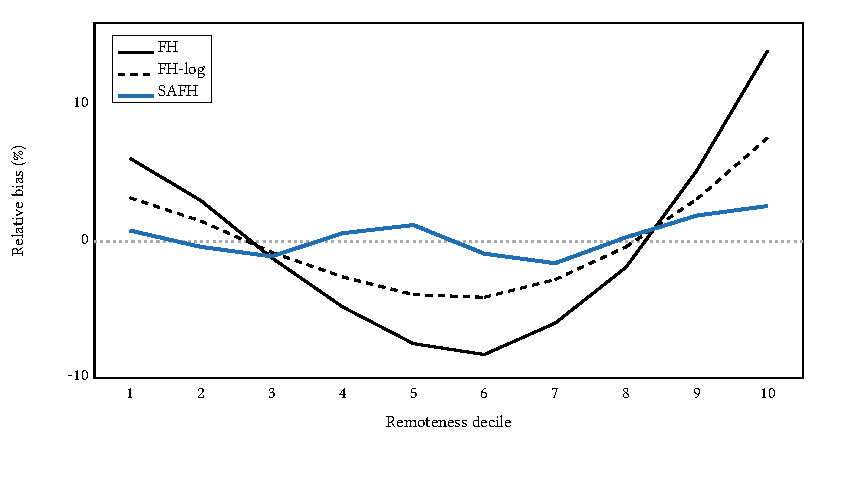
\includegraphics[width=0.85\textwidth]{figures/sim_bias.pdf}
\caption{Average relative bias of the FH, FH-log and SAFH estimators by decile
of the remoteness index, scenario 9 (concave mean function, $m = 100$, low
area-level variance).}
\label{fig:bias}
\end{figure}

The bootstrap intervals for SAFH achieved close to nominal coverage in all
scenarios, with an average coverage of 94.1\% and no scenario below 94.5\%.
Coverage was also stable across districts: Figure~\ref{fig:coverage} shows the
district-specific coverage rates for scenario 9, which lie between 93.2\% and
96.4\% with no systematic pattern in remoteness or sample size. Intervals based
on the naive MSE estimator, by contrast, had an average coverage of only 89.7\%
for $m = 50$.

\begin{figure}[t]
\centering
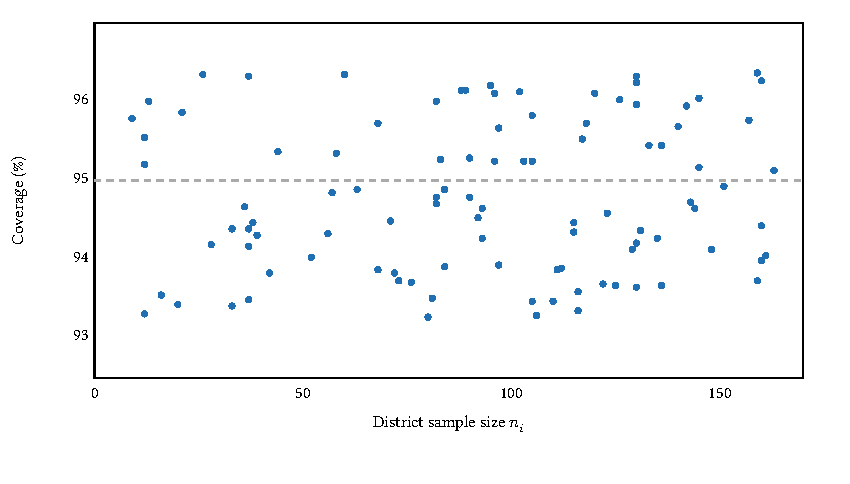
\includegraphics[width=0.85\textwidth]{figures/sim_coverage.pdf}
\caption{District-specific coverage of nominal 95\% SAFH bootstrap intervals
against district sample size, scenario 9.}
\label{fig:coverage}
\end{figure}

Table~\ref{tab:width} reports the average interval width by district sample
size. As expected, the average width of the SAFH intervals increases from
0.214 for districts with fewer than 20 sampled children to 0.081 for districts
with at least 100 sampled children, reflecting the larger weight $\hat w_i$
given to more precise direct estimates. The width of the SAFH intervals is on
average 6\% larger than that of the FH intervals, which is the price paid for
estimating the spline component, but this increase is concentrated in districts
with fewer than 20 sampled children.

\begin{table}[t]
\centering
\caption{Average width of nominal 95\% bootstrap intervals by district sample
size $n_i$, scenario 9.}
\label{tab:width}
\begin{tabular}{lrrr}
\toprule
District sample size & Districts (\%) & FH & SAFH \\
\midrule
$n_i < 20$           & 22 & 0.198 & 0.214 \\
$20 \le n_i < 50$    & 41 & 0.154 & 0.163 \\
$50 \le n_i < 100$   & 26 & 0.112 & 0.118 \\
$n_i \ge 100$        & 11 & 0.079 & 0.081 \\
\bottomrule
\end{tabular}
\end{table}
